%%
%  ******************************************************************************
%  * #file    Szablon_raportu_EN_Latex.tex
%  * #author  Adrian Wójcik   adrian.wojcik(at)put.poznan.pl
%  *          
%  * #commit  Patryk Kościk   koscikpatryk(at)gmail.com
%  *          Modified the template for Projekt przejsciowy purposes          
%  *          
%  *
%  * #commit  Patryk Kościk   koscikpatryk(at)gmail.com
%  *          Zupełnie przewrócono na łeb formatke po taktycznym wyjasnieniu          
%  *          
%  * #version 1.1
%  * #date    09-Mar-2022
%  * #brief   PROJPRZEJ
%  *
%  ******************************************************************************
%%  
\documentclass[11pt, a4paper]{article}

\usepackage{SM_template}

% Wypełnijcie te dyrektywy zgodnie z waszym tematem
%
% \lab      -> NAZWA CZUJNIKA,          np.: 'DHT22'
% \comment  -> Króciutki opis co to,    np.: 'Cyfrowy czujnik temperatury'
% \author   -> Autor dokumentu          np.: Patryk Kościk
%
% Pamiętajcie o zmianie ścieżki w \addbibresourcue (!)

\lab{Niestandardowy moduł LM35DZ}
\comment{Moduł analogowego czujnika temperatury}
\author{Dawid Sobczak}
\addbibresource{bib/LM35DZ.bib}
%
% Początek dokumentu
%
\begin{document}

%
% Strona tytułowa
%
\mainpage{LM35DZ/moduł_lm35dz.jpg}
\newpage

\section*{Opis elementu}
Sensorem składającym się na opisywany moduł jest analogowy czujnik temperatury z rodziny LM35: LM35DZ LP 3-Pin TO-92. Sensor posiada trzy złącza: zasilanie, masa oraz temperatura przedstawiona w woltach. Sensor może być zasilany napięciem w zakresie od $+4$ do nawet $+30$ wolt, oferuje pomiar wartości temperatury w zakresie $(-55,+150)$ stopni Celsjusza z dokładnością $\pm 0.5$ stopnia.\\

Wzór określający zależność napięcia od temperatury wygląda następująco:
\begin{equation}
    V_{OUT} = 10 \cdot T \left[ \frac{mV}{°C}\cdot °C\right],
    \label{wzor}
\end{equation}
Gdzie:
\begin{itemize}
    \item $T$ - to temperatura w stopniach Celsjusza.
\end{itemize}
%(kondensator C1 - 123nF).
%%%%%%%%%%%%%%%%%%%%%%%%%  TWO IMAGES SIDE BY SIDE  %%%%%%%%%%%%%%%%%%%%%%%%%%%%%
\vspace{0.25cm}
\begin{figure}[h]
\centering
%%%%%%%%%%%%%%%%%%%%%%%%%%%%%%%%%%%%%%%%%%%%%%%%%%%%%%%%%%%%%%%%%%%%%%%%%%%%%%%%%
\begin{subfigure}{.5\textwidth}
\centering
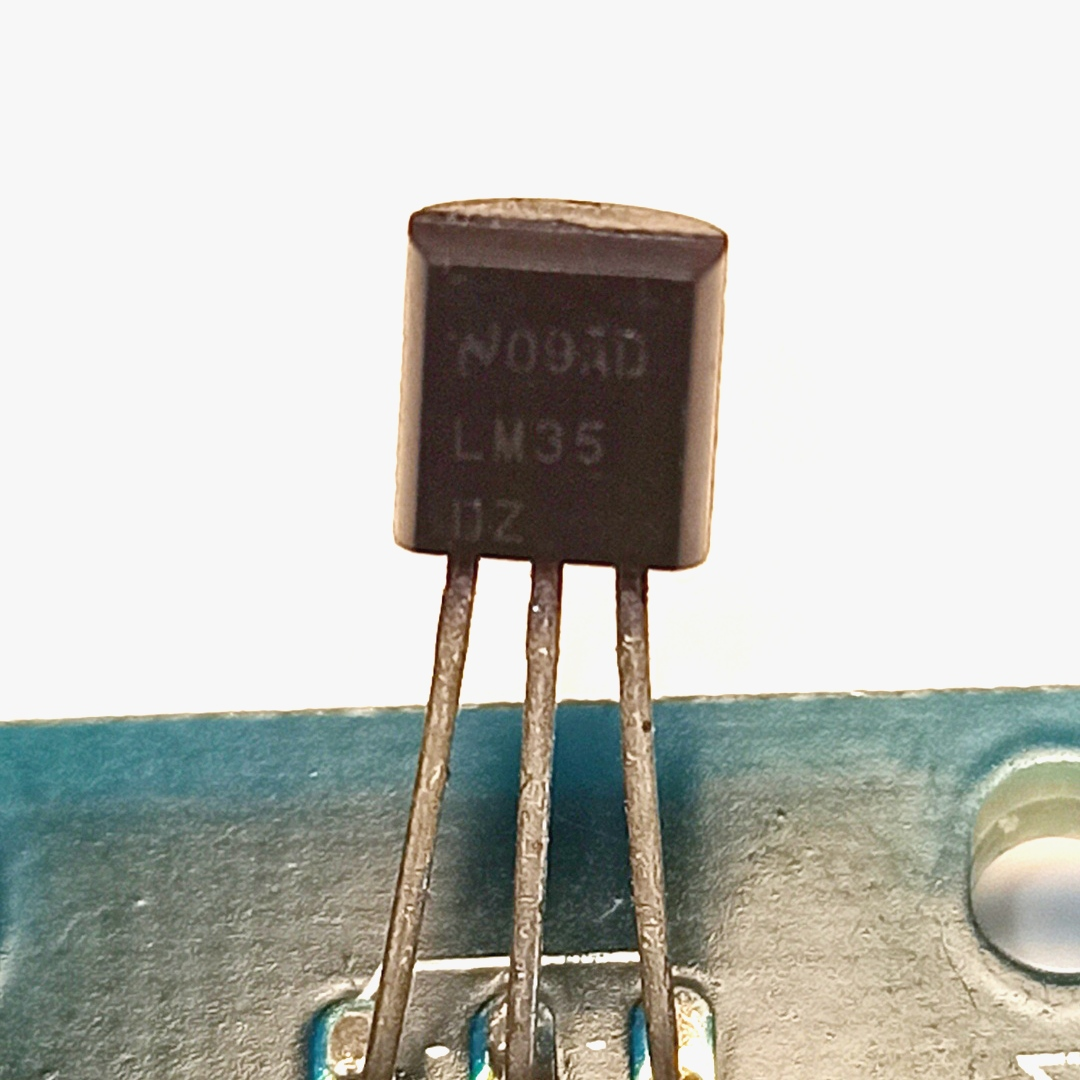
\includegraphics[width=.7\linewidth]{fig/LM35DZ/lm35dz_zdjecie.jpg}
\caption{Sensor LM35DZ - zdjęcie}
\label{fig:_zdjecie_elementu}
\end{subfigure}%
%%%%%%%%%%%%%%%%%%%%%%%%%%%%%%%%%%%%%%%%%%%%%%%%%%%%%%%%%%%%%%%%%%%%%%%%%%%%%%%%%
\begin{subfigure}{.5\textwidth}
\centering
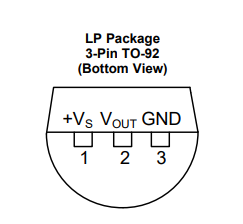
\includegraphics[width=.7\linewidth]{fig/LM35DZ/lm35_lp_schemat.PNG}
\caption{\centering Wyprowadzenia sensora LM35DZ w pakiecie LP 3-Pin TO-92 - schemat}
\label{fig:_zasada_dzialania_elementu}
\end{subfigure}
%%%%%%%%%%%%%%%%%%%%%%%%%%%%%%%%%%%%%%%%%%%%%%%%%%%%%%%%%%%%%%%%%%%%%%%%%%%%%%%%%
% \caption{PODPIS}
\label{fig:element}
\end{figure}
\vspace{0.25cm}
%%%%%%%%%%%%%%%%%%%%%%%%%  TWO IMAGES SIDE BY SIDE  %%%%%%%%%%%%%%%%%%%%%%%%%%%%%
% \subsection{Opis modułu} REPLACE SUBSECTION WITH 1CM VSPACE
\vspace{0.75cm}
%%%%%%%%%%%%%%%%%%%%%%%%%  TWO IMAGES SIDE BY SIDE  %%%%%%%%%%%%%%%%%%%%%%%%%%%%%
\begin{figure}[h]
\centering
%%%%%%%%%%%%%%%%%%%%%%%%%%%%%%%%%%%%%%%%%%%%%%%%%%%%%%%%%%%%%%%%%%%%%%%%%%%%%%%%%
\begin{subfigure}{.5\textwidth}
\centering
\includegraphics[width=.7\linewidth]{fig/LM35DZ/moduł_lm35dz.jpg}
\caption{Moduł czujnika temperatury - zdjęcie}
\label{fig:_zdjecie_modulu}
\end{subfigure}%
%%%%%%%%%%%%%%%%%%%%%%%%%%%%%%%%%%%%%%%%%%%%%%%%%%%%%%%%%%%%%%%%%%%%%%%%%%%%%%%%%
\begin{subfigure}{.5\textwidth}
\centering
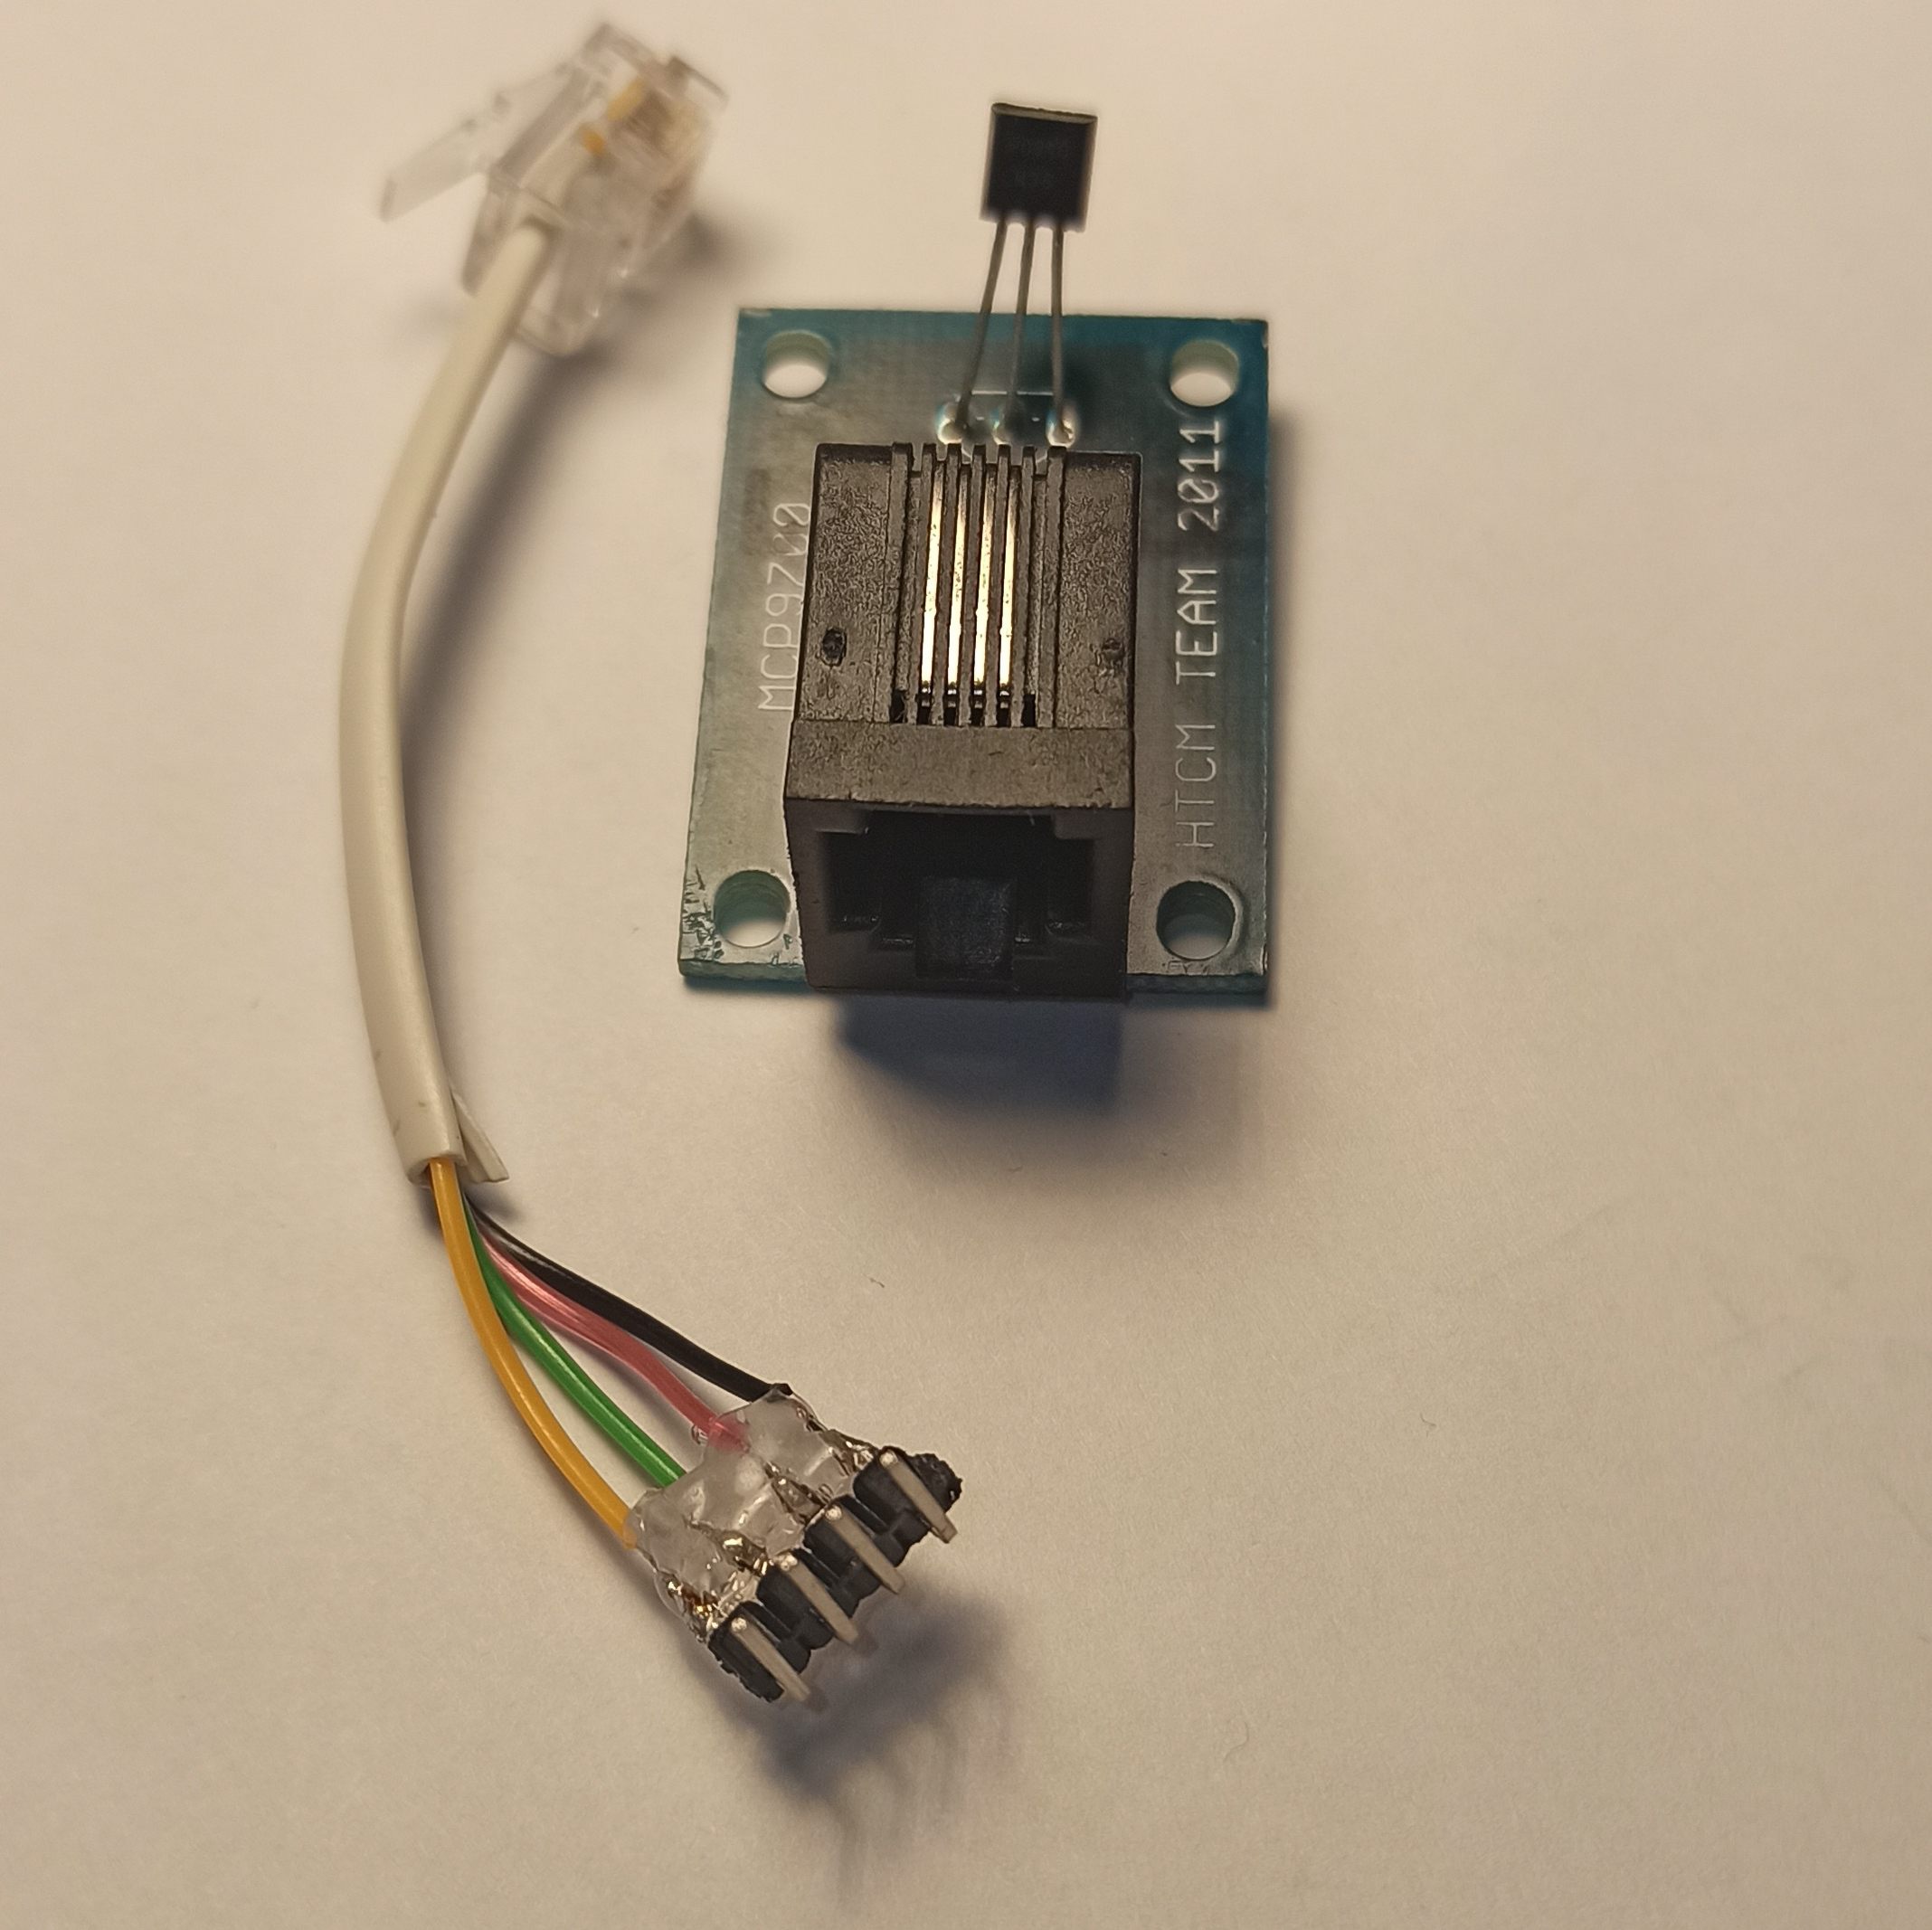
\includegraphics[width=.7\linewidth]{fig/LM35DZ/modul.jpg}
\caption{Złącza modułu (gniazdo RJ11) wraz z kablem}
\label{fig:_schemat_modulu}
\end{subfigure}
%%%%%%%%%%%%%%%%%%%%%%%%%%%%%%%%%%%%%%%%%%%%%%%%%%%%%%%%%%%%%%%%%%%%%%%%%%%%%%%%%
\label{fig:modul}
\end{figure}
\vspace{0.5cm}
%%%%%%%%%%%%%%%%%%%%%%%%%  TWO IMAGES SIDE BY SIDE  %%%%%%%%%%%%%%%%%%%%%%%%%%%%%

\vspace{0.5cm}
Moduł to specjalna plytka PCB z wlutowanym sensorem LM35DZ, kondensatorem filtrującym oraz złączem w postaci gniazda RJ11.
\newpage
\begin{figure}[h]
    \centering
    \includegraphics[width=0.5\textwidth]{fig/LM35DZ/moduł_schemat_elektryczny.PNG}
    \caption{Kompletny schemat elektryczny modułu}
    \label{fig:polaczenie_ukladu}
\end{figure}
\newpage
\section{Użycie modułu}
\subsection{Bez mikrokontrolera}
Najprostszą aplikacją modułu jest podłączenie go do zasilania $+5$ [V] oraz masy, a następnie zmierzenie wartości napięcia pomiędzy pinem określonym jako $V_{OUT}$, a masą oraz oszacowanie wartości temperatury korzystając z wzoru (\ref{wzor}).

\vspace{0.5cm}
% TUTAJ FOTY ODNOSNIE TEGO
%%%%%%%%%%%%%%%%%%%%%%%%%  TWO IMAGES SIDE BY SIDE  %%%%%%%%%%%%%%%%%%%%%%%%%%%%%
\vspace{0.25cm}
\begin{figure}[h]
\centering
%%%%%%%%%%%%%%%%%%%%%%%%%%%%%%%%%%%%%%%%%%%%%%%%%%%%%%%%%%%%%%%%%%%%%%%%%%%%%%%%%
\begin{subfigure}{.5\textwidth}
\centering
\includegraphics[width=.9\linewidth]{fig/LM35DZ/25_test.jpg}
\caption{\centering Wskazanie multimetru dla temperatury pokojowej (około 25 stopni Celsjusza)}
\label{fig:_uklad_woltomierz_otw}
\end{subfigure}%
%%%%%%%%%%%%%%%%%%%%%%%%%%%%%%%%%%%%%%%%%%%%%%%%%%%%%%%%%%%%%%%%%%%%%%%%%%%%%%%%%
\begin{subfigure}{.5\textwidth}
\centering
\includegraphics[width=.9\linewidth]{fig/LM35DZ/30_test.jpg}
\caption{\centering Wskazanie multimetru przy lekkim ogrzaniu otoczenia czujnika temperaturą ludzkiego ciała}
\label{fig:_uklad_woltomierz_zmk}
\end{subfigure}
%%%%%%%%%%%%%%%%%%%%%%%%%%%%%%%%%%%%%%%%%%%%%%%%%%%%%%%%%%%%%%%%%%%%%%%%%%%%%%%%%
% \caption{PODPIS}
\label{fig:woltomierz}
\end{figure}
\vspace{0.25cm}
%%%%%%%%%%%%%%%%%%%%%%%%%  TWO IMAGES SIDE BY SIDE  %%%%%%%%%%%%%%%%%%%%%%%%%%%%%
Określenie temperatury jest banalnie proste, gdyż wskazanie mulitimetra wystarczy podzielić przez 10.
\vspace{0.5cm}
\subsection{Mikrokontroler}
Aplikacja modułu wymaga połączenie mikrokontrolera z modułem w sposób opisany w tabeli (\ref{tab:tab1}) znajdującej się poniżej.

\vspace{0.5cm}
\begin{table}[h!]
    \centering
    \begin{tabular}{|c|c|c|c|} 
        \hline
        \multicolumn{2}{|c|}{NUCELO-F746ZG} & \multicolumn{2}{c|}{Moduł LM35}  \\ 
        \hline
        Etykieta & Port i numer pinu       & Nr pinu & Etykieta           \\ 
        \hline
        GND      & -                    & 1       & GND             
        \\
        \hline
        D42      & PA3                    & 2       & $V_{OUT}$          
        \\
        \hline
        -      & -                      & 3       & N.C.              \\
        \hline
        +5V      & -                       & 4       & $+V_s$              \\
        \hline
    \end{tabular}
    \caption{Połącznie pomiędzy modułem i mikrokontrolerem}
    \label{tab:tab1}
\end{table}

Dodatkowe schematy połączeń i konfiguracja
mikrokontrolera została opisana w sekcji \texttt{Suplement \#1}. Zawiera tam się również kod języka
C + HAL, pozwalający na obsługę modułu.

\newpage
\begin{figure}[h]
    \centering
    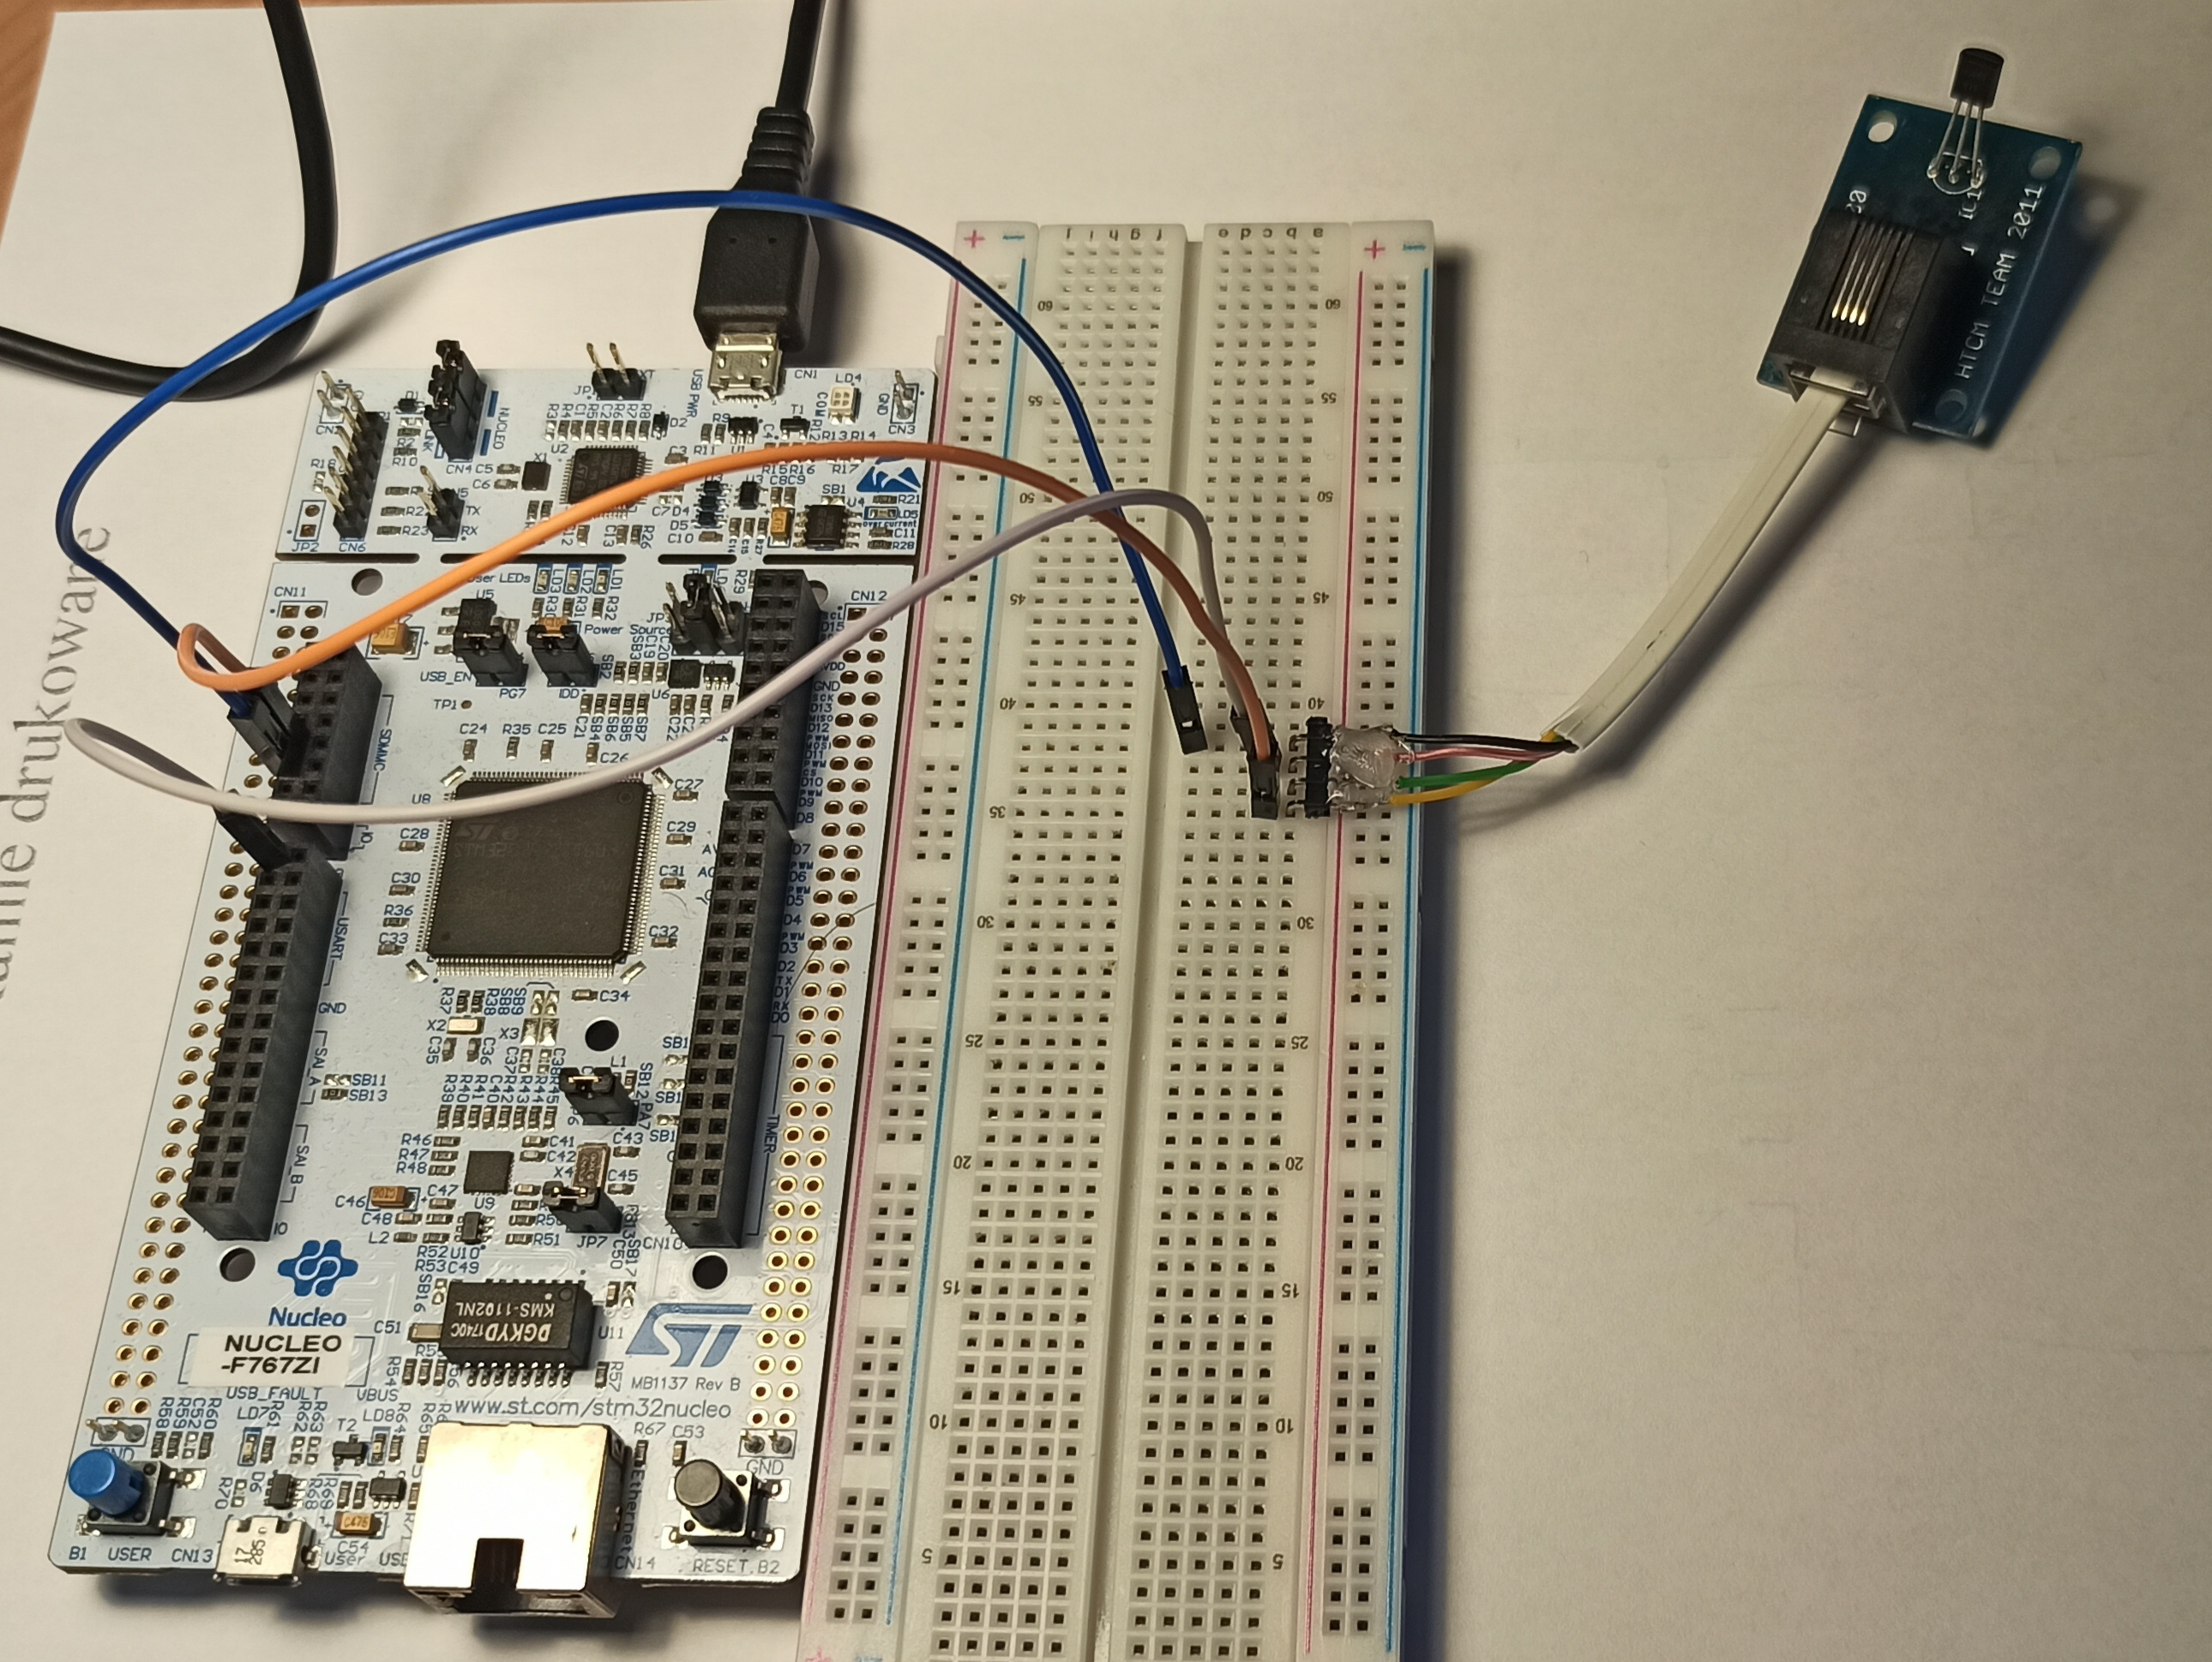
\includegraphics[width=0.5\textwidth]{fig/LM35DZ/polaczenie.jpg}
    \caption{Połączenie układu - zdjęcie}
    \label{fig:polaczenie_ukladu}
\end{figure}
\begin{figure}[h]
    \centering
    \includegraphics[width=0.5\textwidth]{fig/LM35DZ/moduł_schemat_polaczenia.PNG}
    \caption{Połączenie układu - schemat}
    \label{fig:polaczenie_ukladu}
\end{figure}
\vspace{0.5cm}
Działanie modułu z sensorem analogowym w aplikacji z mikrokontrolerem zostało zaprezentowane na materiałe wideo zawartym w \texttt{\cite{yt1}}.

\newpage
\printbibliography[heading=bibintoc]

\end{document}